\documentclass{sig-alternate}

\begin{document}
\conferenceinfo{OZCHI}{'14, Dec 2-5, 2014, Sydney, Australia}

\title{Visualising a Live Coding Arts Process}

\numberofauthors{3}
\author{
\alignauthor Arrian Purcell\\
       \affaddr{Research School of}\\
       \affaddr{Computer Science, CECS}\\
       \affaddr{Australian National University}\\
       \email{u5015666@anu.edu.au}
\alignauthor Henry Gardner\\
       \affaddr{Research School of}\\
       \affaddr{Computer Science, CECS}\\
       \affaddr{Australian National University}\\
       \email{henry.gardner@anu.edu.au}
\alignauthor Ben Swift\\
       \affaddr{Research School of}\\
       \affaddr{Computer Science, CECS}\\
       \affaddr{Australian National University}\\
       \email{ben.swift@anu.edu.au}
}

\maketitle
\begin{abstract}
  This paper describes an empirical study of source code visualisation
  as a means to communicate the programming process in ``live coding''
  computer music performances. Following an exploratory field study of
  a live-coding performance at an arts festival, two different
  interaction-driven visualisation techniques were incorporated into a
  live coding system. We then performed a more controlled laboratory
  study to evaluate the visualisations' contributions to the audience
  experience, with emphasis on the (self-reported) experiential
  dimensions of \emph{understanding} and \emph{enjoyment}. Both
  software visualisation techniques enhanced audience enjoyment, while
  the effect on audience understanding was more complex. We conclude
  by suggesting how these visualisation techniques may be used to
  enhance the audience experience of live coding.
\end{abstract}

\category{H.5.2}{Information Interfaces and Presentation}{User Interfaces}[Evaluation/methodology]

\terms{Design, Experimentation}

\keywords{Live coding, musical performance, software visualisation}

\section{Introduction}

``Show us your screens\ldots Code should be seen as well as heard'',
declares the draft manifesto of ``TOPLAP''~\cite{Toplap}, an
international organisation devoted to the artistic performance
practice of ``live coding''. In live coding, computer code is written
in front of a live audience to generate music and visuals in real
time. The ``show us your screens'' rhetoric underscores the need for
authenticity to distinguish this artform from similar (but non-live)
computational arts practices.

But what actually is the benefit of the live coder showing their
screen? In a live coding performance, non-expert live coding audience
members spend much of their time staring at raw (usually text-based)
computer code. In a live coding performance, including those described
in this paper, the computer code is central to the audience
experience, being projected onto large screens behind the performer.
Until now, little empirical study has been undertaken to gauge an
audience's response to that computer code and whether, from an
audience perspective, code really should be ``seen as well as heard''.

Traditional approaches to source code visualisation
(see~\cite{Novais2013} for a review) often focus on the structure of
the source code (e.g. visualising complex object/class relationships)
rather than the \emph{process} of programming. In a process-oriented
activity such as live coding, different code visualisation techniques
are thought to be necessary~\cite{McLean2010a,Magnusson2013}.
However, until now, academic treatments of code visualisations in live
coding have adopted theoretical and descriptive approaches, and have
not included empirical evaluation of the visualisation techniques.

In this paper, we examine the audience's experience of displayed code
and visualisations during live coding performances to see whether
code-driven visualisations might improve both the audience enjoyment
and the audience understanding of these performances. Our
investigations commenced with a field study at a contemporary-arts
festival and subsequently included a controlled, laboratory-based
audience study.

\section{Exploratory Field Study}

Immediately following a live-coding performance at the \emph{You Are
Here} arts festival in Canberra, Australia, in March 2014, we asked
audience members to fill out a survey regarding their perception of,
and response to, the projected computer code. Each audience member was
asked to indicate which of five curves best represented the way that
their (self-reported) ``\emph{enjoyment}" and their
``\emph{understanding}" (of the relationship between the visuals and
the music) over time through the performance (an example of one of
these curves can be seen in Figure~\ref{fig:understanding-over-time}).
The curve trajectories in this survey allowed for ``high'',
``medium'', and ``low'' levels of enjoyment/understanding for the
(self-determined) ``beginning'', ``middle'' and ``end'' phases of the
performance. Other survey questions addressed the ``liveness'' of the
performance (c.f.~\cite{Auslander}) and whether the projected code was
confusing.\\

\subsection{Field Study Results}

Of the thirteen survey responses received (roughly $80\%$ of the total
audience), six audience members reported a high level of enjoyment
throughout the whole performance, while the remaining seven responses
reported alternating levels of enjoyment. No audience members
indicated a low level of enjoyment throughout the performance.

Only two of the thirteen respondents indicated that they understood
the relationship between the code projections and the music throughout
the performance. Three of the six respondents who reported a high
level of enjoyment throughout the performance also indicated an
increase in understanding (from low to high) as the performance
progressed, although a Chi-square analysis revealed no significant
relationship between enjoyment and understanding. Nine of the thirteen
respondents stated that the code projection provided a sense of
liveness to the performance and the remainder stated that viewing the
code had no effect on their sense of liveness. Four respondents felt
that the code projections were confusing, five felt that they were not
confusing, and four did not answer the question.

Taken as a whole, the results of this small field study were
salutatory concerning the benefit of ``seeing as well as hearing''
code during a live coding performance. The majority of the audience
felt that the code made the performance seem more ``live''. However, a
minority stated that they found the projections confusing and only a
very small number of respondents claimed to have actually understood
what the programmer was doing. We were intrigued by the three
respondents whose understanding increased through the performance and
whose enjoyment remained high, and we wished to test whether
augmenting code projections with additional visualisations might give
rise to similar responses across the wider audience.

\section{Laboratory Study}

\begin{figure}
\centering
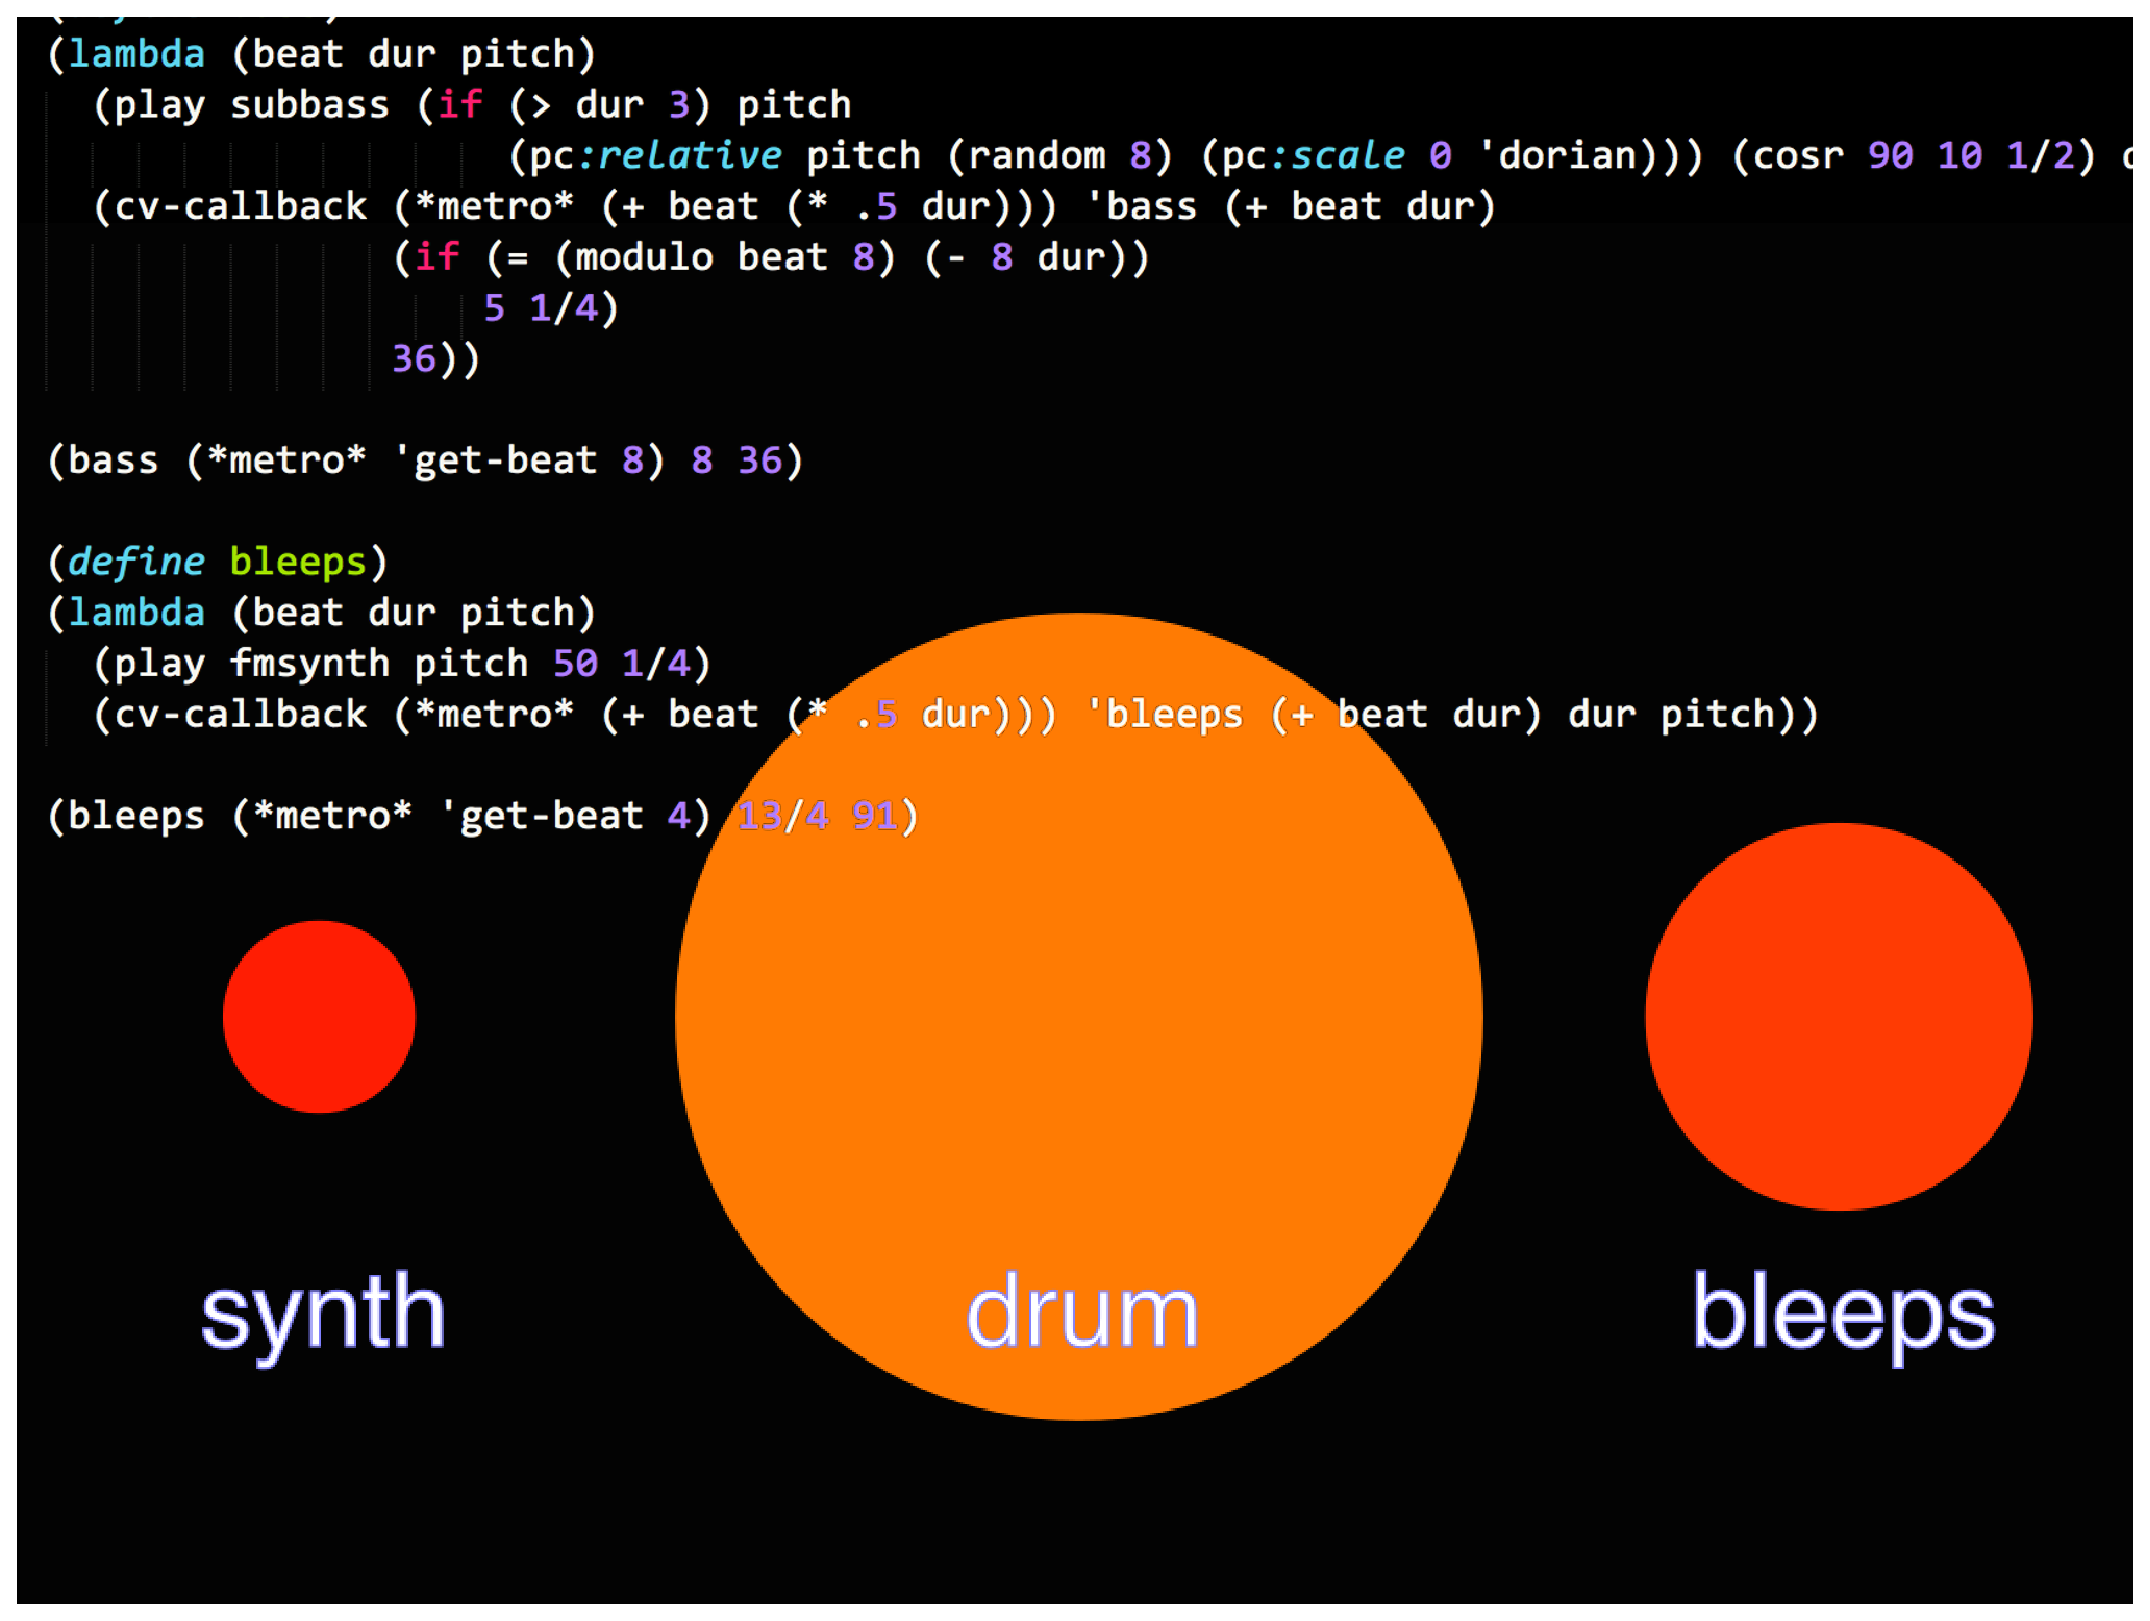
\epsfig{file=didactic-vis-overlay.eps, width=\columnwidth}
\caption{An example didactic visualisation (all
  figures best viewed in colour).}
\label{fig:didactic-visualisation}
\end{figure}

\begin{figure}
\centering
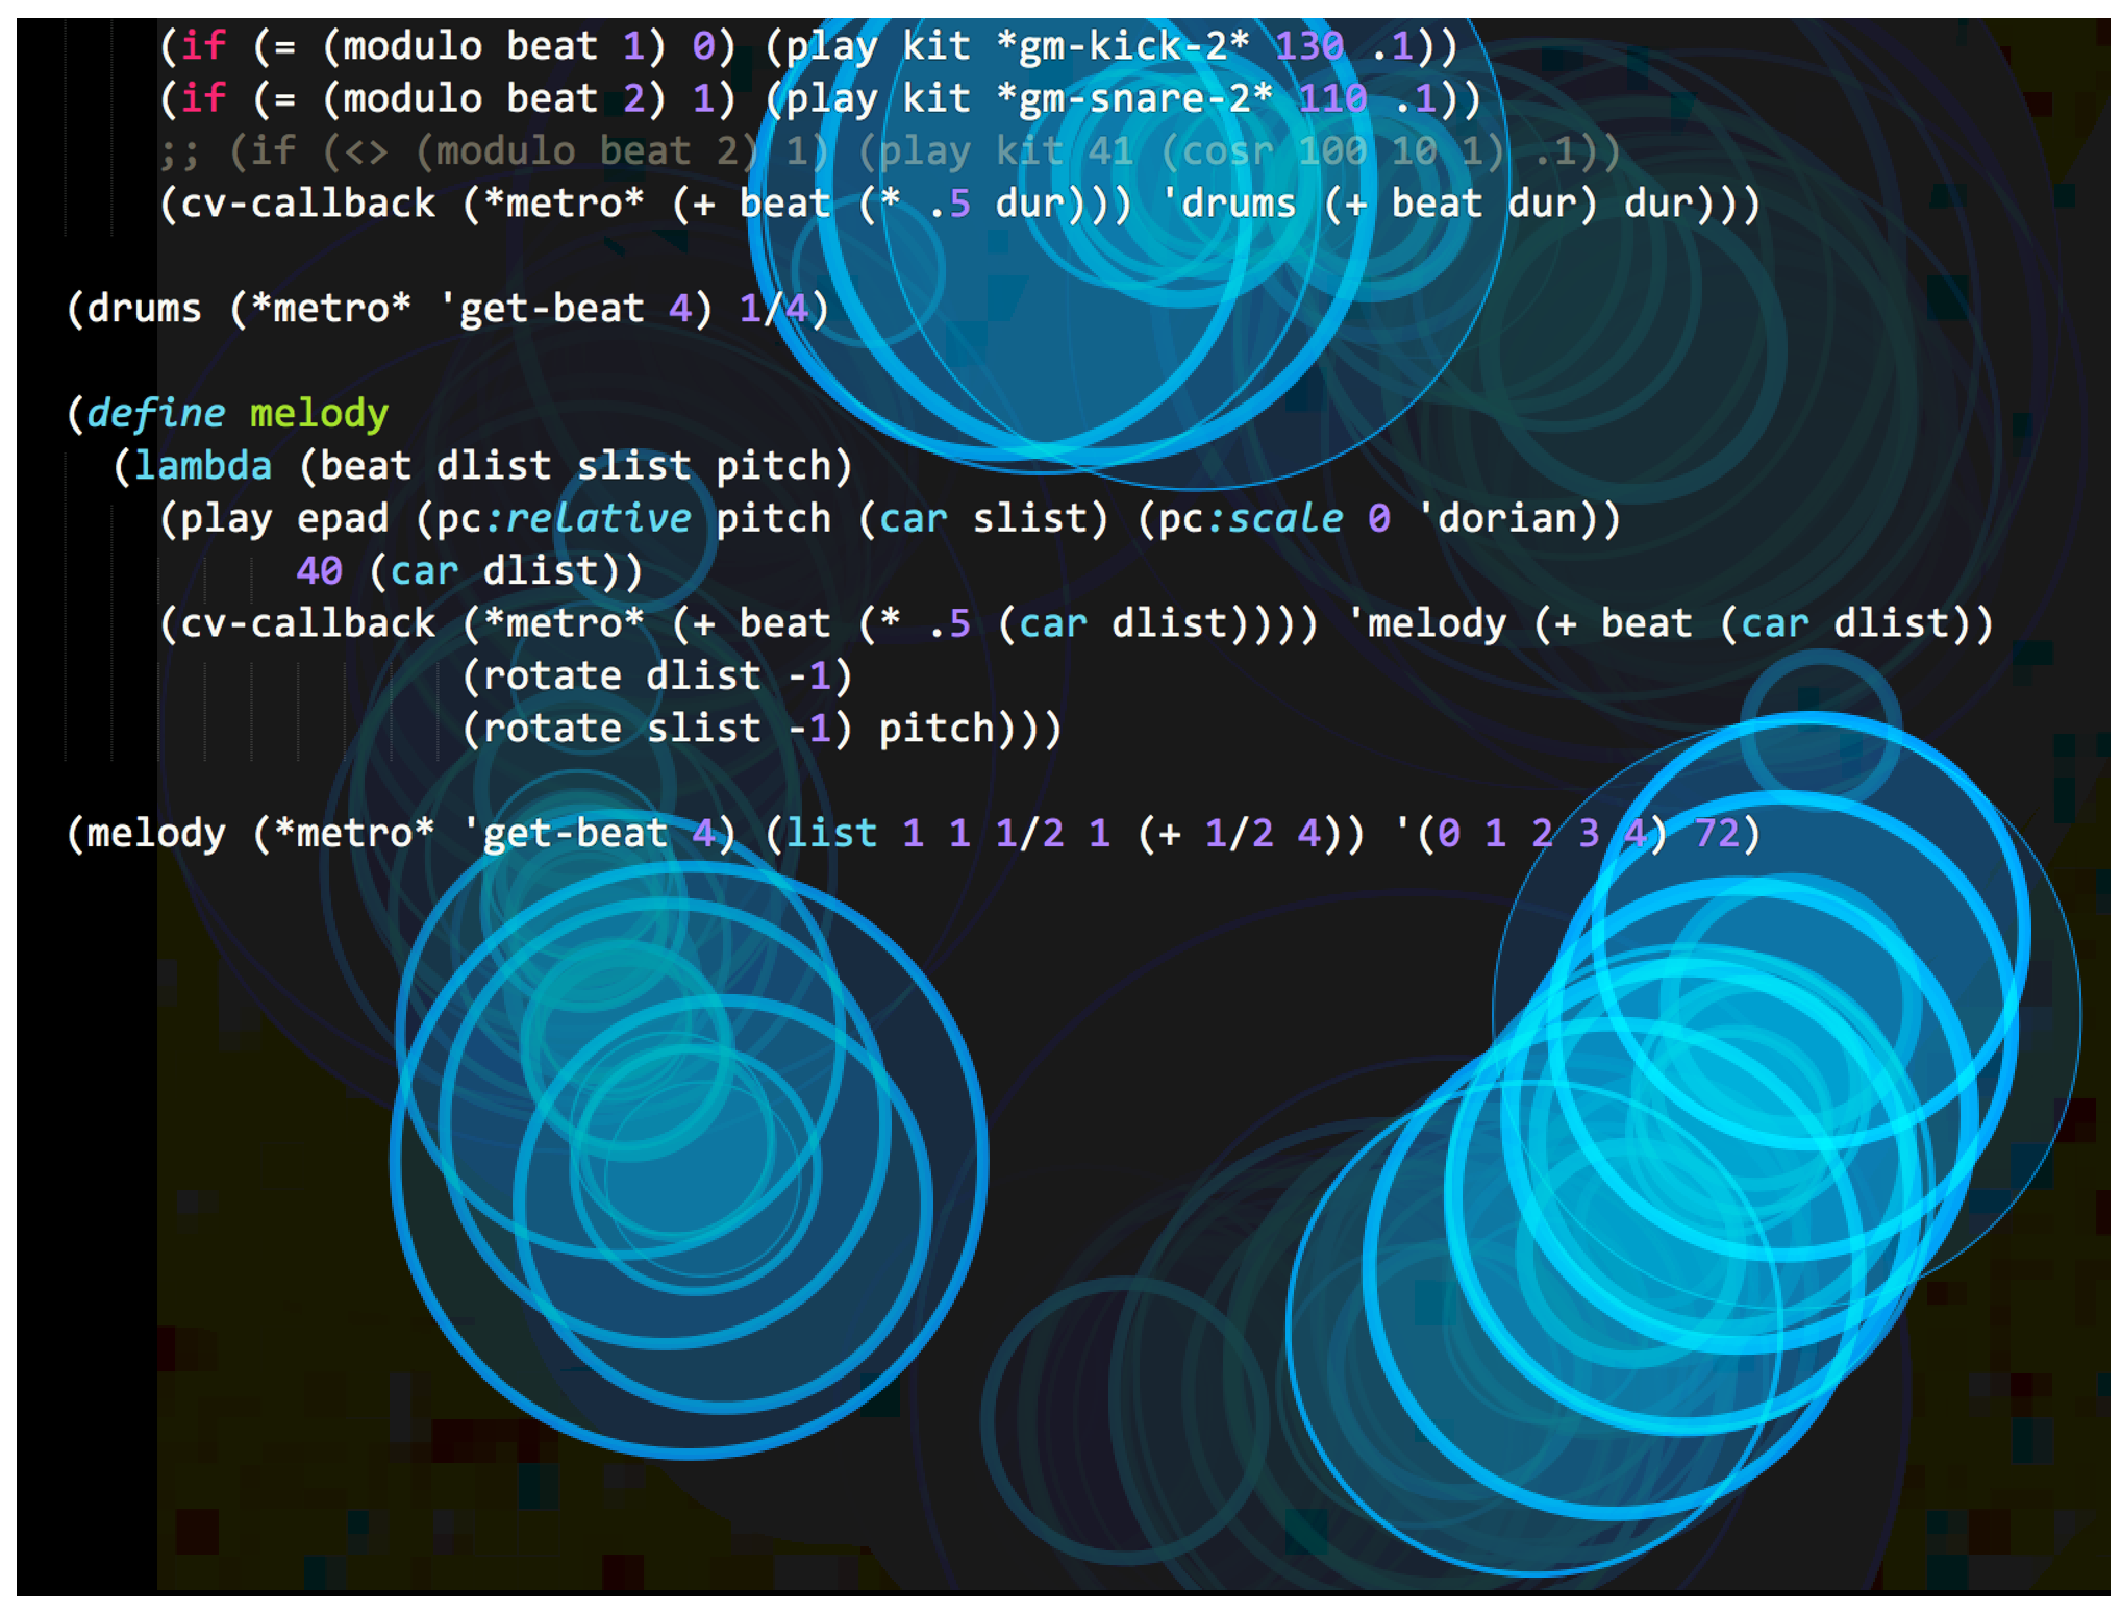
\epsfig{file=aesthetic-vis-overlay.eps, width=\columnwidth}
\caption{An example aesthetic visualisation.}
\label{fig:aesthetic-visualisation}
\end{figure}

A laboratory study was conducted to test the impact of accompanying
visualisations on audience understanding and enjoyment of live coding.
Music visualisation is an extremely rich and open-ended task, so to
guide the development of our visualisations, we used the concepts of
understanding and enjoyment to develop two new code visualisations
which we termed ``\emph{didactic}" and ``\emph{aesthetic}".

The \emph{didactic} visualisation (shown in
Figure~\ref{fig:didactic-visualisation}) attempted to communicate
\emph{information} about the actions of the programmer, prominently
displaying the \emph{names} of the active (source code) functions and
the ``time until next execution'' for each function (which is
particularly relevant in a time-sensitive programming context such as
music making). Bright colours and solid shapes were used to ensure
constant visibility and to communicate the intention of the underlying
code.

The \emph{aesthetic} visualisation technique, was designed to react to
the programmer's activity in a more abstract way, to maximise
aesthetic appeal~\cite{Cawthon2007} and to engage the audience's
interest. Although still based on the source code and the live coder's
edits, the generation of shapes was driven by instrument volume and
synchronised with the musical beat. The emphasis for the aesthetic
visualisation was on the artistic appeal of the visuals (see
Figure~\ref{fig:aesthetic-visualisation}), including more variety in
visual structure and colour. Like the didactic condition, the
aesthetic visualisations proceeded through four stages, based on the
number of active functions (instruments), but these visuals had no
textual labels and they moved and interacted with each other over the
entire projected scene.

Our hypothesis was the didactic visualisation would result in enhanced
audience understanding through the performance. In contrast, we
predicted that the aesthetic visualisations would more positively
influence audience enjoyment.

\subsection{Experimental Design}

\begin{figure*}
\centering
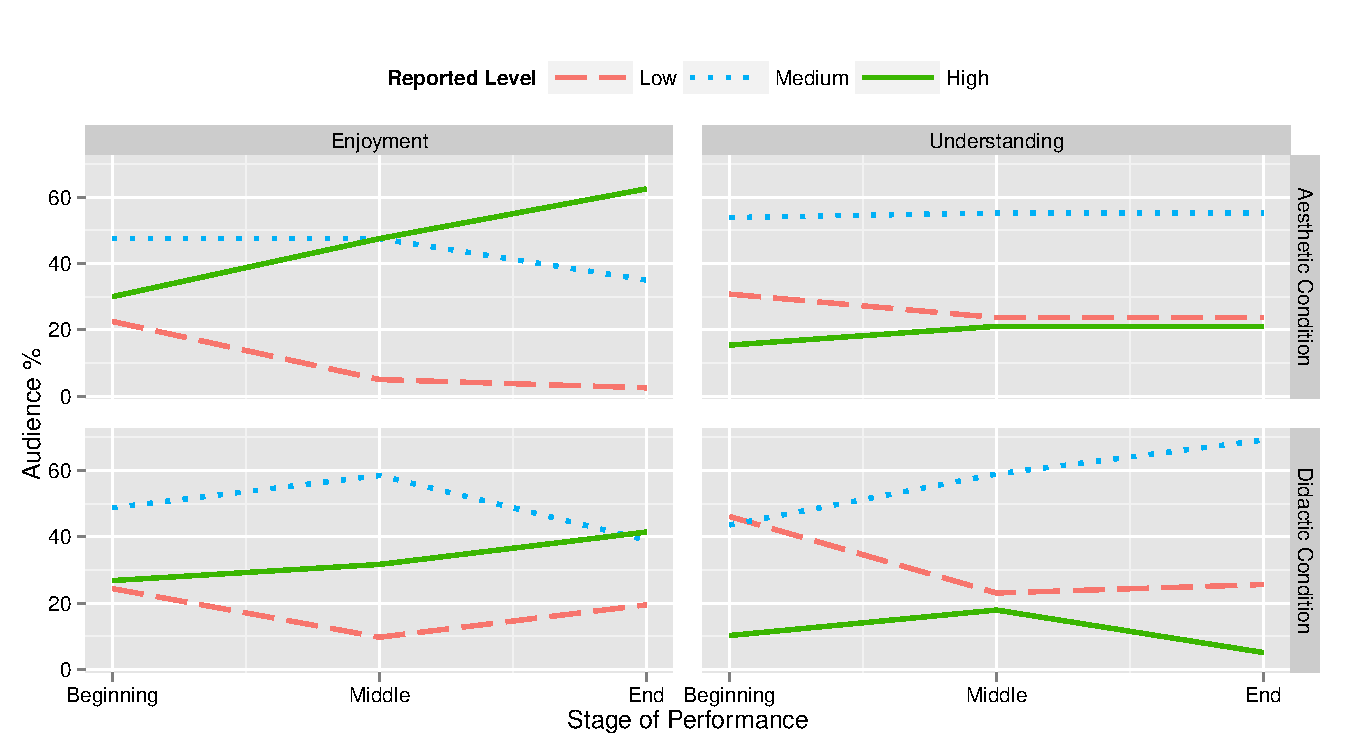
\epsfig{file=dimension-condition-2x2.pdf, width=\textwidth}
\caption{Percentage of the audience reporting high (green) and low
 (red) enjoyment and understanding over the beginning, middle and end
stages of the performances for the aesthetic and didactic conditions.
The remaining percentage not shown here reported a level of medium
enjoyment or understanding.}
\label{fig:enjoyment-understanding}
\end{figure*}

To assess the impact of these two visualisation techniques on audience
understanding and enjoyment, we conducted a laboratory study. Two
independent audiences ($N=19+22=41$), recruited through an on-campus
advertisement, each watched a live coder perform two ten-minute
``sets'': one accompanied by the didactic visuals, and one with the
aesthetic. The order of presentation of the two visual conditions was
swapped between the groups. The improvisational nature of a live
coding performance makes ``controlled'' experiments difficult, but the
live coding artist attempted (as much as possible) to perform with
similar musical aesthetic and quality across all performances.

Over the course of these performances, each audience member completed
a survey consisting of four sections: demographic information, their
opinion of the first musical piece, their opinion of the second
musical piece and questions regarding the performance overall. Similar
to the first field trial, the questionnaire primarily focussed on
self-reported levels of ``enjoyment'' and ``understanding''. But, in
this case, these levels were tallied as categorical variables (low,
medium and high) rather than being related to curves such as that
shown in Figure~\ref{fig:understanding-over-time}). There was also a
free-format question for suggested improvements to the visualisations.

Following this laboratory study, a
video-cued-recall~\cite{Suchman:1992tk} interview was conducted with
the live coder using a video of the performance.

\subsection{Laboratory Study Results}

Of the $41$ audience participants, $66\%$ were male, $76\%$ were aged
between 18 and 32, and $78\%$ had never seen a live coding performance
before. In the following discussion of the results we refer to global
statistical measures of the data, categorical trends as shown in
Figure~\ref{fig:enjoyment-understanding} and detailed analysis of
population cohorts which are not shown here for the sake of brevity. A
significance level of $0.05$ was used for the Chi-squared analysis.

\subsubsection{Enjoyment}

Overall, the majority of the participants reported that \emph{both}
visualisation conditions had a positive effect on their
\textbf{enjoyment}: $76\%$ stated that the aesthetic visualisations
improved their enjoyment and $56\%$ stated that the didactic
visualisations improved their enjoyment. No significant difference
between the visualisation types  was found
($\chi^2=3.7733,df=2,p=0.1516$).

Participants were asked to rate their enjoyment during the
(self-determined) ``beginning'', ``middle'' and ``end'' of the
performances. The aesthetic visualisation resulted in a larger
percentage (around $60\%$) of the audience reporting high enjoyment
during the middle of the performance compared to the didactic
visualisation (around $40\%$). Notably, only a very small percentage
reported low enjoyment for the aesthetic visualisations during the
middle and end of the performance in comparison to the didactic
visualisations.

\subsubsection{Understanding}

In response to a specific survey question, $37\%$ of participants
stated that overall, the didactic visualisations ``helped them to
\textbf{understand} the code'', compared to $12\%$ of participants for
the aesthetic visualisations. This was a significant difference
between the visualisation conditions ($\chi^2=7.1986,df=2,p=0.02734$).

Again, participants were asked to rate their understanding during the
(self-reported) ``beginning'', ``middle'' and ``end'' of the
performance. The aesthetic visualisation resulted in a smaller
percentage of the audience (around $30\%$) reporting low understanding
during the beginning of the performance compared to the didactic
visualisations (around $45\%$). This trend continued through the
middle but equalised by the end of the performance.\\

\subsection{Discussion}

The overall effect of visualisations on enjoyment was high for both
the aesthetic and didactic visualisations. Reported enjoyment of the
aesthetic visualisations was higher than for the didactic
visualisations.

The trends for understanding are complex. The smaller number of high
responses for understanding throughout the performances perhaps
indicate a higher cognitive load for understanding the didactic
visualisations themselves during the initial stages of the
performance. In fact, features of the didactic visualisation were
reported to \emph{confuse} some members of the audience, despite their
stated aim of \emph{assisting} audience understanding. One audience
member even stated that they ``found them distracting'' and that they
``preferred just to read the code''.

The video-cued-recall interview with the live coder indicated that the
experience of the visualisations by the live coder and by audience was
fundamentally different. While many members of the audience reported
that they drifted between focussing on the music, focussing on the
visualisations and focussing on the code, the live coder reported that
their focus was purely on the code and the music, rarely drifting. In
one particular section of the interview, the live coder stated: ``I
definitely wasn't paying attention to them [the visualisations] on the
day. In fact I tune them out as best I can because I am just trying to
focus on the code''. By contrast, one audience member stated that
``you could see the code being written and the visualisations helped
to show when a piece of code started working''. Another audience
member stated that ``the visualisations were interesting but
distracting''. When asked if the visualisations were distracting, the
live coder stated: ``Ah, no. In general I'm just so focussed on the
code''.

\begin{figure}
\centering
\fbox{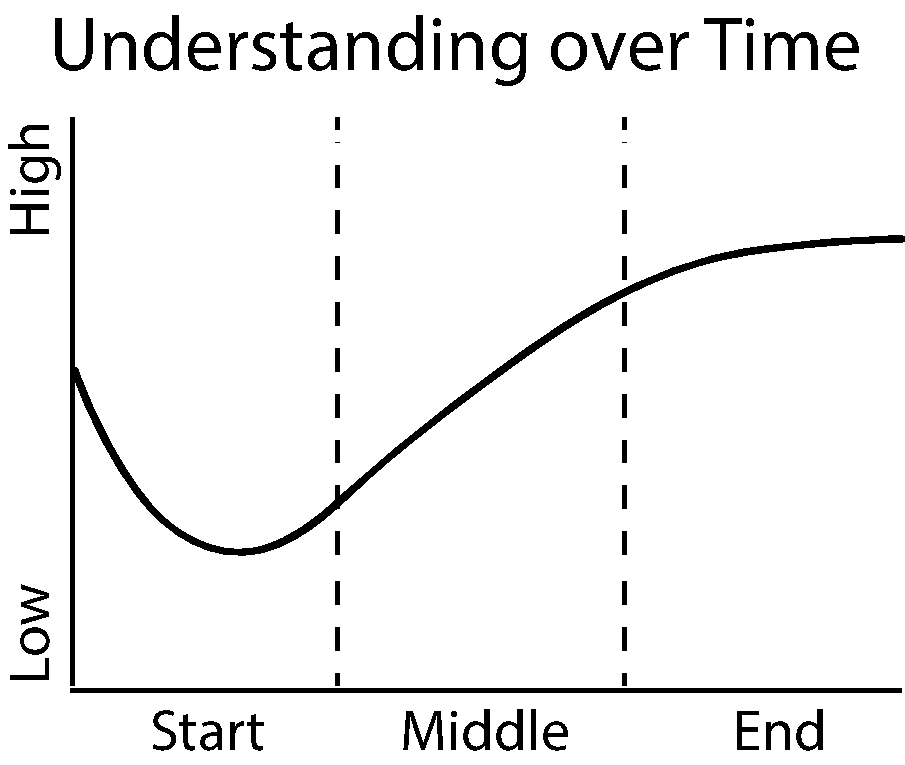
\epsfig{file=understanding-over-time.pdf, width=1.0\columnwidth}}
\caption{An example of one of the curves provided to the audience
during the initial field study. A total of five curve options were
provided. The survey question asked the participants to: ``circle the
image that best represents your understanding of the relationship
between the visuals and the music through the performance.''}
\label{fig:understanding-over-time}
\end{figure}

\section{Conclusion}

In this first empirical study of audience perception of code
visualisation in live coding, we have identified an opportunity for
real-time code visualisations to help improve the audience experience
of a live-coding computer-music performance. With few exceptions, our
initial survey of a live coding performance at an arts festival
revealed a generally low to medium level of audience self-reported
understanding throughout that performance (although almost half the
survey respondents indicated a high level of enjoyment throughout).

In the laboratory study, a comparison of two prototype code
visualisations indicated that both visualisations seemed to help with
enjoyment. Significantly, more audience members reported that our
didactic visualisations helped with understanding but overall trends
for both enjoyment and understanding throughout the performances were
complex. There are indications of a higher cognitive load for the
didactic visualisations than the aesthetic visualisations and this may
have influenced audience responses to them.

In a future extension of this work, design lessons from both
visualisation types could be combined together to produce live coding
visualisations which target both aesthetics and understanding of the
live coding process. These visualisations could then be compared with
the baseline ``no visualisation'' condition in an audience experiment.
There are also opportunities to vary the nature of the visualisations
over the course of a performance.

Over sixty years ago, the media theorist Marshall McLuhan stated that
``The business of art is no longer the communication of thoughts or
feelings which are to be conceptually ordered, but a direct
participation in an experience. The whole tendency of modern
communication\ldots is towards participation in a process, rather than
apprehension of concepts.''~\cite{McLuhan} Our hope is that future
developments in visualisations for live coding may bring audiences
further into the \emph{process} of a highly-skilled live coding
artist.

\bibliographystyle{abbrv}

\begin{thebibliography}{1}

\bibitem{Auslander}
P.~Auslander.
\newblock {\em {Liveness: Performance in a Mediatized Culture}}.
\newblock Routledge, second edition, 2008.

\bibitem{Cawthon2007}
N.~Cawthon and A.~V. Moere.
\newblock {The Effect of Aesthetic on the Usability of Data Visualization}.
\newblock {\em 2007 11th International Conference Information Visualization (IV
  '07)}, pages 637--648, July 2007.

\bibitem{Magnusson2013}
T.~Magnusson.
\newblock {Algorithms as Scores: Coding Live Music}.
\newblock {\em Leonardo Music Journal}, 21:19--23, 2011.

\bibitem{McLean2010a}
A.~Mclean, D.~Griffiths, N.~Collins, and G.~Wiggins.
\newblock {Visualisation of live code}.
\newblock {\em Visualisation and the Arts}, pages 1--5, 2010.

\bibitem{McLuhan}
M.~McLuhan.
\newblock {Letter to Harold Adam Innis, March 14 1951}.
\newblock In E.~McLuhan and F.~Zingrone, editors, {\em Essential McLuhan},
  page~73.

\bibitem{Novais2013}
R.~L. Novais, A.~Torres, T.~S. Mendes, M.~Mendon\c{c}a, and N.~Zazworka.
\newblock {Software evolution visualization: A systematic mapping study}.
\newblock {\em Information and Software Technology}, 55(11):1860--1883, Nov.
  2013.

\bibitem{Suchman:1992tk}
L.~A. Suchman and R.~H. Trigg.
\newblock {Understanding practice: video as a medium for reflection and
  design}.
\newblock pages 65--90, 1992.

\bibitem{Toplap}
Toplap.
\newblock {Toplap Manifesto}.
\newblock http://toplap.org/wiki/ManifestoDraft, 2010.

\end{thebibliography}

\end{document}
